\documentclass{article}
\usepackage{graphicx} % Required for inserting images
\usepackage{amsmath} % Required for some math elements
\usepackage{hyperref}
\title{\textsc{Term Project}}
\title{\textbf{Synthetic Spectra for Interstellar
        Molecules in LTE and non-LTE regimes}}
\author{Maitrey Sharma}
\date{April 23, 2024}
\begin{document}

\maketitle
\begin{abstract}
This work presents a code which can calculate the intensities of 
atomic and molecular lines produced in a uniform medium, 
based on statistical equilibrium calculations involving 
collisional and radiative processes and including radiation 
from background sources to infer physical and chemical 
parameters such as temperature, density, and molecular abundances.
\end{abstract}
\section{Introduction}
Consider a mono-atomic or singly-charged chemical species in gaseous state with
\(N\) energy levels defined as \(E_i\) with \(i = 1 \ldots N\) in ascending
order. Pertaining to the temperature this chemical species exists at, each
level will have certain occupation or population. These occupation numbers can
change due to collisions between neighboring molecules and if the environment
is sufficiently dense and temperatures are sufficiently high, this population
distribution can be deemed as thermal and can be expressed as
\begin{equation}\label{eq:1}
    \dfrac{N_j}{N_i} = {e}^{-(E_j - E_i)/k_B T}
\end{equation}
Here, \(N_i\) (and \(N_j\)) represents the level occupation number density of state
\(i\) (and \(j\)), \(k_B\) is the Boltzmann constant and \(T\) is the temperature of the
gas. This thermal distribution is basis for the condition of \textit{local thermodynamic
    equilibrium} or LTE.\@ In other words, the mean free path of the (excited) molecules
is much, much less than the scales at which the temperature varies in the medium.

Equation~\ref{eq:1} can be modified to include the degeneracies of states through
statistical weights, which results in
\begin{equation}
    \dfrac{N_j}{N_i} = \dfrac{g_j}{g_i} {e}^{-(E_j - E_i)/k_B T}
\end{equation}
where \(g_i = 2l+ 1\), \(l\) being the orbital angular momentum of electron in state
\(i\). And finally, we can obtain the fractional occupational numbers \(n_i\) using the
partition function \(Z(T)\) as
\begin{equation}
    n_i = \dfrac{1}{Z(T)} g_i {e}^{-E_i / k_B T}
\end{equation} 

\section{Radiative Transfer}
Now, transitions between levels can also be facilitated by 
the emission or absorption of a photon. 
This is called a radiative transition, 
or a spectral line transition.
\begin{equation}
    \dfrac{d I_{\nu}}{ds} = j_{\nu} - \alpha_{\nu} I_{\nu}
\end{equation}
where \(I_{\nu}\) is the specific intensity defined as the 
amount of energy passing through a surface normal to the path, 
per unit time, surface, bandwidth (measured here in frequency 
units), and solid angle.\ \(j_{\nu}\) and \(\alpha_{\nu}\) are
the local emission and excitation coefficients. This can be solved
to obtain
\begin{equation}
    I_{\nu} = I_{\nu} (0) {e}^{\tau_{\nu}} + \int_0^{\tau_{\nu}}
    S_{\nu} (\tau'_{\nu}) {e}^{-(\tau_{\nu}-\tau'_{\nu})} d\tau'_{\nu}
\end{equation}
where \(I_{\nu} (0)\) is the background radiation entering the medium.
To calculate the emission and excitation coefficients, we require the
Einstein coefficients \(A_{ij}\) and \(B_{ij}\) along with a function 
called \textit{line profile} \(\phi(\nu)\) which basically defines the susceptibility 
of the transition to photons of frequency \(\nu\).

In the case of LTE, radiative transfer can be performed by using the
following data
\begin{enumerate}
    \item A \textit{line list} This is a list (usually in ASCII format) 
    in which for each line the \(A_{ij}\), \(E_i\), \(\nu_{ij}\),
    \(g_i\), \(g_j\) are given.
    \item A \textit{partition function table} as a function of
    temperature.
\end{enumerate}
But if we were to perform a non-LTE radiative transfer, we will need
\begin{enumerate}
    \item A \textit{level list} in which for each level the
    \(E_i\) and \(g_i\) are given.
    \item \textit{Collisional rates} \(C_{ij}\) between each pair of levels
    at different temperatures.
    \item A \textit{line list} but this time containing, for each line, 
    the index \(i\) of the upper and
    \(j\) of the lower level, where these indices refer to the level list mentioned above.
    Along with, of course, \(A_{ij}\) and line profile information.
\end{enumerate}
As collisional rates difficult to measure in lab, for most of the 
astrophysically relevant species, only LTE radiative transfer is
possible.

\subsection{The Problem of non-LTE transfer}
If the level populations \(n_i\) are known, 
the radiative transfer equation can be solved exactly. 
In particular, under LTE conditions, knowledge of the 
kinetic gas temperature \(T_{\text{kin}}\) allows the 
determination of 
\(n_i\) by virtue of the Boltzmann equation.
For many interstellar and circumstellar media, 
the density is too low to attain LTE, but 
statistical equilibrium (SE) can often be assumed.
Under the condition of SE, for every level \(i\) we 
demand that the rate at which atoms/molecules are being
(de-) excited out of level \(i\) is equal to the rate at 
which level \(i\) is being re-populated by
(de-) excitation from other levels:
\begin{equation}\label{eq:2}
    \sum_{j > i} n_j A_{ji} - \sum_{j < i} n_i A_{ij} + 
    \sum_{j} [n_j C_{ji} -n_i C_{ij}] = 0
\end{equation}
This must be true for all levels \(i\) and therefore,
Equation~\ref{eq:2} constitutes a coupled set of \(N_{\text{lev}}\)
linear equations with \(N_{\text{lev}}\) unknowns, or in other words,
a matrix equation.

\subsection{Lambda Iteration and Accelerated Lambda Iteration}
The Lambda iterative scheme is defined as follows used in order
to solve a coupled set of equations:
\begin{enumerate}
    \item Make an initial guess for the mean intensity
    \item  Integrate the formal transfer equation along a large number of rays, such that
    close to every point \(x\) a sufficient number of rays pass by that we can make an
    approximate calculation of the mean intensity\label{item:2}
    \item Compute mean intensity at all locations, thereby 
    computing the scattering emissivity
    \item Go back to~\ref{item:2}, until we find a converged solution to
    mean intensity.
\end{enumerate}

We can rewrite~\ref{eq:2} by including the mean intensity \(J_{ij}\) as
\begin{equation}\label{eq:3}
    \begin{split}
        &\sum_{j > i} [n_j A_{ji} + (n_j B_{ji} - n_i B_{ij})J_{ji}] \\
        & - \sum_{j < i} [n_i A_{ij} + (n_i B_{ij} - n_j B_{ji}) J_{ij}] \\
        & + \sum_{j \neq i} [n_j C_{ji} - n_i C_{ij}] = 0
    \end{split}
\end{equation}
By defining something called the Lambda operator as
\begin{equation}
    J_{\nu} = \Lambda [S_{\nu}]
\end{equation}
which basically acts as a function which computes the mean intensity \(J\)
at some point \(\mathbf{x}\) knowing what the source function \(S_{\nu} (\mathbf{x'})\)
is for all \(\mathbf{x'}\). In principle, the \(\Lambda_{ij}\) can be defined as
\begin{equation}
    \Lambda_{ij} = \dfrac{1}{4 \pi} \int d \nu \oint d \Omega \phi_{ij}
    (\nu, \mathbf{x}, \mathbf{n}) \Lambda_{\nu, \mathbf{n}}
\end{equation}
where \(\Lambda_{\nu, \mathbf{n}}\) is the angle-dependent Lambda operator.
Equation~\ref{eq:3} then becomes
\begin{equation}\label{eq:4}
    \begin{split}
        &\sum_{j > i} [n_j A_{ji} + (n_j B_{ji} - n_i B_{ij})
        \Lambda_{ji}[S_{ji}]] \\
        & - \sum_{j < i} [n_i A_{ij} + (n_i B_{ij} - n_j B_{ji})
        \Lambda_{ij}[S_{ij}]] \\
        & + \sum_{j \neq i} [n_j C_{ji} - n_i C_{ij}] = 0
    \end{split}
\end{equation}
Now lambda iteration just involves the iteration between solving the set
of equations in~\ref{eq:3} for given \(J_{ij}\), and computing \(J_{ij}\)
for given \(n_i\). Using~\ref{eq:4}, we can write
\begin{equation}\label{eq:5}
    \begin{split}
        &\sum_{j > i} [n_j^{m+1} A_{ji} + (n_j^{m+1} B_{ji} - n_i^{m+1} B_{ij})
        \Lambda_{ji}[S_{ji}^m]] \\
        & - \sum_{j < i} [n_i^{m+1} A_{ij} + (n_i^{m+1} B_{ij} - n_j^{m+1} B_{ji})
        \Lambda_{ij}[S_{ij}^m]] \\
        & + \sum_{j \neq i} [n_j^{m+1} C_{ji} - n_i^{m+1} C_{ij}] = 0
    \end{split}
\end{equation}
where \(m\)-index is the iteration counter.  After each iteration you solve the coupled
set of linear equations~\ref{eq:5} to obtain new set of level populations.

We can improve Lambda iteration by splitting of the \(\Lambda\)-operator.
\begin{equation}
    \Lambda_{ij} = \Lambda^{\ast}_{ij} + (\Lambda_{ij} - \Lambda^{\ast}_{ij})
\end{equation}
as form of separating out the diagonal (or tridiagonal) part of the operator
matrix. This gives rise to the accelerated Lambda iteration scheme or ALI and
can be summarized as
\begin{equation}\label{eq:6}
    \begin{split}
        &\sum_{j > i} [n_j^{m+1} A_{ji}(1-\Lambda^{\ast}_{ji})
        + (n_j^{m+1} B_{ji} - n_i^{m+1} B_{ij})
        (\Lambda_{ji} - \Lambda^{\ast}_{ji})
        [S_{ji}^m]] \\
        & - \sum_{j < i} [n_i^{m+1} A_{ij}(1-\Lambda^{\ast}_{ij})
        + (n_i^{m+1} B_{ij} - n_j^{m+1} B_{ji})
        (\Lambda_{ij} - \Lambda^{\ast}_{ij})
        [S_{ij}^m]] \\
        & + \sum_{j \neq i} [n_j^{m+1} C_{ji} - n_i^{m+1} C_{ij}] = 0
    \end{split}
\end{equation}

\subsection{The Escape Probability Scheme}
Now that we have a mathematical framework to efficiently solve the coupled system
of equations, we can return to the problem at hand and analyze it scientifically
as well to see if we can make some further approximations. Even with the above
iterative schemes, for inhomogeneous or geometrically complex objects, 
extensive calculations with many grid points are required. However, if only the global
properties of the source are of interest then we can introduce a geometrically
averaged escape probability \(\beta\), the probability that a photon will escape the medium from where it was created.
This probability depends only on the optical depth \(\tau\) and is 
related to the intensity within the medium, ignoring background 
radiation and any local continuum, through
\begin{equation}
    J_{\nu_{ul}} = S_{\nu_{ul}} (1 - \beta)
\end{equation}
We have included three kinds of geometries in our implementation. The first one
comes from Sobolev's Large Velocity Gradient (LVG) approximation for an extending spherical
shell. For this case, the probability is given by
\begin{equation}
    \beta_{\text{LVG}} = \dfrac{1}{\tau} \int_0^{\tau} e^{\tau'} d\tau'
    = \dfrac{1 - e^{-\tau}}{\tau}
\end{equation}
The second geometry is that of a uniform static sphere and escape probability
for it is given by
\begin{equation}
    \beta_{\text{sphere}} = \dfrac{1.5}{\tau}
    \left[1 - \dfrac{2}{\tau^2} + \left(
        \dfrac{2}{\tau} + \dfrac{2}{\tau^2}
    \right) e^{-\tau}
    \right]
\end{equation}
And lastly, we have a plane-parallel slab geometry, applicable for shocks
\begin{equation}
    \beta_{\text{slab}} = \dfrac{1 -e^{-3\tau}}{3\tau}
\end{equation}

\section{Description of the Code}
\subsection{Input to the code}
\begin{enumerate}
    \item The code leverages the Leiden Atomic and Molecular Database (LAMDA)
    database to get the required data required for non-LTE radiative transfer.
    Therefore, first input is the LAMDA file for the molecule/species one is interested
    in.
    \item The geometry of the system, as described in the last section to get the
    correct escape probability scheme.
    \item A function to obtain the background radiation. By default, we use
    the cosmic microwave background, which means basically radiation corresponding
    to the \(T = 2.73\) K.
    \item The kinetic temperature of the source. This will be used to calculate the
    corresponding uprates and downrates of collisional events between particles at
    different energy levels. Uprates and downrates are linked through detailed
    balance equation.
    \item Densities of the collisional partners. Collisional partners are often
    the most abundant species such has the hydrogen molecule (present in two forms
    as spin isomers: ortho and para).
    \item The (total) column density of the molecule one is interested in. Column density
    is basically the integrated number density of a molecular species along a column
    formed by the line of sight.
    \item The full-width half-maximum of the line profile. Line profiles can be Gaussian
    or rectangular.
\end{enumerate}
\subsection{Output of the code}
\begin{enumerate}
    \item The code displays results for all transitions. These results include
    quantum numbers, the upper and lower energy levels, excitation temperature,
    frequency and wavelength.
    \item The line optical depth, defined as the optical depth of the equivalent rectangular line shape.
    \item Fractional populations (occupational numbers) for each energy level.
    \item The line intensity, defined as the Rayleigh-Jeans equivalent temperature.
    \item Once the above items are calculated, few extra inputs can be supplied to calculate
    more relevant quantities. For example, flux can be computed by providing distance to the
    observer, radius of the source (as sources are assumed to be spherical or slab-like)
    and the solid angle subtended by the source. The last one is what links this to actual
    observations through telescopes.
    \item Finally, we can obtain the final synthetic spectrum by using the given input
    parameters along with the source function.
\end{enumerate}
\section{Results}
\begin{figure}
	\centering
	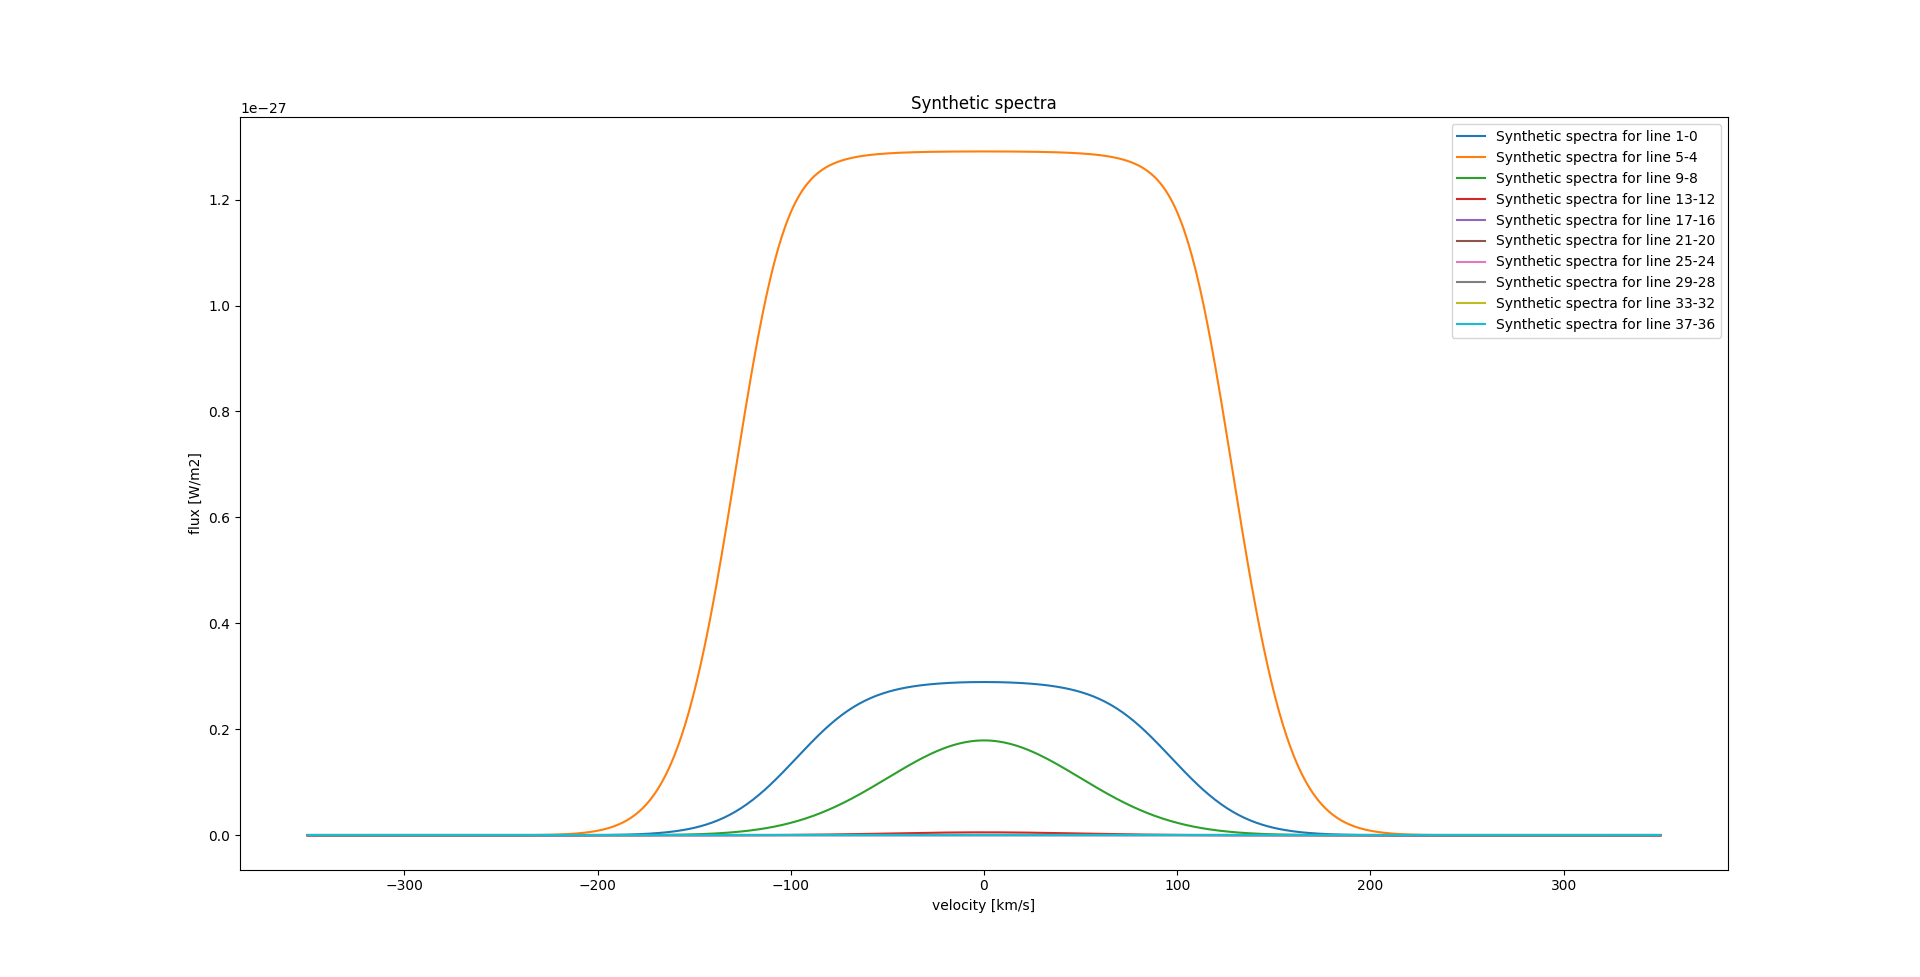
\includegraphics[scale=0.25]{Figure_1.png}
	\caption{Synthetic spectrum in the non-LTE regime.}
\end{figure}

\nocite*{}
\bibliography{ref}
\bibliographystyle{plainurl}
\end{document}
